\documentclass{article}
\usepackage[ruled,vlined,linesnumbered]{algorithm2e}
\usepackage{algpseudocode}
\usepackage{amsmath}
\usepackage{amsthm}
\usepackage{graphicx}
\usepackage{subfigure}
\usepackage{float}
\usepackage{amsmath }
\usepackage{amsfonts }
\usepackage{pdfpages}
\usepackage{epsfig}
\usepackage{graphicx}
\usepackage{arydshln}
\usepackage{verbatim}
\usepackage{subfigure}
\usepackage{enumerate}
\usepackage{rotating}
\usepackage{threeparttable}
\usepackage{caption}
\usepackage{epsfig}
\usepackage{cite}
\usepackage{tikz}
\usetikzlibrary{shapes}
\usetikzlibrary{shapes.geometric}
\usepackage{geometry}
\geometry{a4paper, top=2.54cm, bottom=2.54cm, left=3.18cm, right=3.18cm}
\theoremstyle{definition}
\newtheorem{prob}{Problem}
\newtheorem{ans}{Answer}
\usepackage[colorlinks,linkcolor=black]{hyperref}
\linespread{1.2}
\begin{document}
	\title{Assignment 5}
	\author{Kailing Wang 521030910356}
	\date{December 5.2022}
	\maketitle
	
	\begin{prob}
		(25 points) [Fair Division Revisited] Suppose we want to allocate $m$ indivisible items to $n$ agents. A $n \times m$ matrix $V=\left[v_{i j}\right]_{i=1, \ldots, n ; j=1, \ldots, m}$ describes agents' preferences over the items, where $v_{i j}$ is the value of item $j$ according to agent $i$ 's preference. We assume agents' valuations are binary, i.e., $v_{i j} \in\{0,1\}$ for any $i$ and $j$. Given a subset $S$ of items, agent $i$ 's value on $S$ is naturally defined by $v_{i}(S)=\sum_{j \in S} v_{i j}$.

		\noindent An allocation $\left(A_{1}, \ldots, A_{n}\right)$ is a partition of $[m]:=\{1, \ldots, m\}$, where $A_{i} \subseteq[m]$ is the set of the items allocated to agent $i$. An allocation is proportional if $v_{i}\left(A_{i}\right) \geq\left\lfloor\frac{1}{n} v_{i}([m])\right\rfloor$ holds for any agent $i$. That is, in a proportional allocation, each agent receives his/her average integer value, rounded down, of the entire item set. For example, if $v_{i j}=1$ for all $i$ and $j$, the average value for each agent is $m / n$, and each agent needs to get at least $\left\lfloor\frac{m}{n}\right\rfloor$ items to guarantee proportionality.
		
		\noindent In this question, we are going to prove the existence of proportional allocations and design an algorithm to find one.
		
		\begin{enumerate}[(a)]
			\item (5 points) Let us first assume, for this moment, that items are divisible. That is, we are allow to fractionally allocate a single item such that an agent gets some portion of it. Show that there exists a fractional allocation such that each agent $i$ receives a value of at least $\frac{1}{n} v_{i}([m])$.
			\item (5 points) Consider the flow network with $m+n+2$ vertices $s, u_{1}, \ldots, u_{n}, w_{1}, \ldots, w_{m}, t$ described as follows. There is a directed edge from $s$ to each $u_{i}$ with capacity $\frac{1}{n} v_{i}([m])$. There is a directed edge from $u_{i}$ to $w_{j}$ with capacity $\infty$ if $v_{i j}=1$. There is a directed edge from each $w_{j}$ to $t$ with capacity 1 . According to Part (a), what is the maximum flow in this network?
			\item (5 points) Now, we modify the network by reducing the capacity of each edge $\left(s, u_{i}\right)$ from $\frac{1}{n} v_{i}([m])$ to $\left\lfloor\frac{1}{n} v_{i}([m])\right\rfloor$. What is the maximum flow in this network?
			\item (5 points) Show that the maximum flow in Part (c) can be made integral. Use this result to show that the proportional allocation always exists even when items are indivisible.
			\item (5 points) Design an algorithm to compute a proportional allocation. 
			
		\end{enumerate}
	\end{prob}
	
	\begin{ans}
		~
		
		\begin{enumerate}[(a)]
			\item If the items are fractional, we can simply divide each item to $n$ pieces and give one piece to each agent regardless of whether he/she wants it or not. This way, the value each agent receives is exactly $\frac{1}{n} v_{i}([m])$ because he/she actually receives $\frac{1}{n}$ portion of each item. 
			
			In fact, we can also throw away the $\frac{1}{n}$ of item $j$ if agent $i$ does not prefer item $j$. This does not change the value he/she gets. 
	
			\item First we prove that this flow network depicts the problem of Part (a). Draw the network as Plot 0. The capacity from $s$ to $u_i$ is the required value we expect that each agent receive. The $\infty$ capacity ensures that all the received value should cost the same amount from $w_i$. If agent $i$ does not prefer item $j$, we don't allocate any of item $j$ to agent $i$. The 1 capacity shows that there is only 1 item for each kind. When dividing the items, we can set the flow on each line at any value so that the items should be fractional, which is the same as what we suppose in Part (a).
			
			\begin{center}
				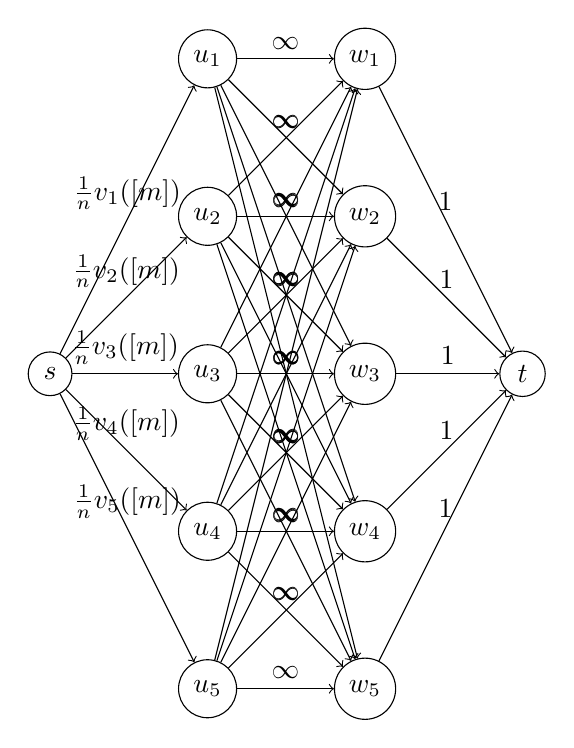
\begin{tikzpicture}
					\node[circle, draw] (s) at (0,0) {$s$};
					\node[circle, draw] (1) at (2,-4) {$u_5$};
					\node[circle, draw] (2) at (2,-2) {$u_4$};
					\node[circle, draw] (3) at (2,0) {$u_3$};
					\node[circle, draw] (4) at (2,2) {$u_2$};
					\node[circle, draw] (5) at (2,4) {$u_1$};
					\node[circle, draw] (w1) at (4,-4) {$w_5$};
					\node[circle, draw] (w2) at (4,-2) {$w_4$};
					\node[circle, draw] (w3) at (4,0) {$w_3$};
					\node[circle, draw] (w4) at (4,2) {$w_2$};
					\node[circle, draw] (w5) at (4,4) {$w_1$};
					\node[circle, draw] (t) at (6,0) {$t$};
					\draw[->] (s) -- (1) node[midway, above] {$\frac{1}{n} v_{5}([m])$};\draw[->] (s) -- (2) node[midway, above] {$\frac{1}{n} v_{4}([m])$};\draw[->] (s) -- (3) node[midway, above] {$\frac{1}{n} v_{3}([m])$};\draw[->] (s) -- (4) node[midway, above] {$\frac{1}{n} v_{2}([m])$};\draw[->] (s) -- (5) node[midway, above] {$\frac{1}{n} v_{1}([m])$};
					\draw[->] (w1) -- (t) node[midway, above] {$1$};\draw[->] (w2) -- (t)node[midway, above] {$1$};\draw[->] (w3) -- (t)node[midway, above] {$1$};\draw[->] (w4) -- (t)node[midway, above] {$1$};\draw[->] (w5) -- (t)node[midway, above] {$1$};
					\draw[->] (1) -- (w1) node[midway, above] {$\infty$};\draw[->] (1) -- (w2) node[midway, above] {$\infty$};\draw[->] (1) -- (w3) node[midway, above] {$\infty$};\draw[->] (1) -- (w4) node[midway, above] {$\infty$};\draw[->] (1) -- (w5) node[midway, above] {$\infty$};
					\draw[->] (2) -- (w1) node[midway, above] {$\infty$};\draw[->] (2) -- (w2) node[midway, above] {$\infty$};\draw[->] (2) -- (w3) node[midway, above] {$\infty$};\draw[->] (2) -- (w4) node[midway, above] {$\infty$};\draw[->] (2) -- (w5) node[midway, above] {$\infty$};
					\draw[->] (3) -- (w1) node[midway, above] {$\infty$};\draw[->] (3) -- (w2) node[midway, above] {$\infty$};\draw[->] (3) -- (w3) node[midway, above] {$\infty$};\draw[->] (3) -- (w4) node[midway, above] {$\infty$};\draw[->] (3) -- (w5) node[midway, above] {$\infty$};
					\draw[->] (4) -- (w1) node[midway, above] {$\infty$};\draw[->] (4) -- (w2) node[midway, above] {$\infty$};\draw[->] (4) -- (w3) node[midway, above] {$\infty$};\draw[->] (4) -- (w4) node[midway, above] {$\infty$};\draw[->] (4) -- (w5) node[midway, above] {$\infty$};
					\draw[->] (5) -- (w1) node[midway, above] {$\infty$};\draw[->] (5) -- (w2) node[midway, above] {$\infty$};\draw[->] (5) -- (w3) node[midway, above] {$\infty$};\draw[->] (5) -- (w4) node[midway, above] {$\infty$};\draw[->] (5) -- (w5) node[midway, above] {$\infty$};
				\end{tikzpicture}
			
			Plot 0: Here I use TIKZ to draw
			\end{center}
			The flow network describes the same problem as problem a. To solve the max flow problem, we can set the flow from $u_i \text{ to } w_j$ to $\frac{1}{n}$ if $v_{ij}$ is 1 and otherwise 0. This way, we have
			$$
			\overunderset{n}{i=1}{\Sigma} f(s\rightarrow u_i)=\overunderset{n}{i=1}{\Sigma} c(s\rightarrow u_i)
			$$
			
			And these concerned edges form a cut of the network. According to the Maximum Flow-Minimum Cut Theorem, this allocation forms a max flow for this problem. The max flow is $\overunderset{n}{i=1}{\Sigma} \frac{1}{n} v_{i}([m])=\frac{m}{n}$.
			\item As what I've explained in Part (b), if we reduce the capacity of edge $(s, u_i)$, we have to reduce the flow on the edges $(u_i, w_j)$ and that of $w_j, t$. Making this reduction is always legal. Since the flow is reduced from the one in Part (b), the flow on edge $(s, u_i)$ is $\lfloor\frac{1}{n}v_i([m])\rfloor$. We get a flow with total value $\lfloor\frac{1}{n}\overunderset{n}{i=1}{\Sigma}v_i( [m])\rfloor$, which equals the cut formed by all the $(s, u_i)$ edges. According to the theorem, the flow is maximum.
			\item In this case, we have to modify the flow network by limiting the flow on edge $(u_i, w_j)$ to be either 0 or 1. We can simply set all these capacities 1. Note that now all the capacities are integers. Under this condition, the result of Edmonds-Karp algorithm will give an integer flow so the flow on $(u_i, w_j)$ is indeed either 0 or 1. The actual modification is that we set the capacity on edge $(u_i, w_j)$ 1. However, in the max flow given by previous problems, the flow on these edges must be smaller than one because $(w_j, t)$ has capacity 1. The max flow for the modified network is still $\lfloor\frac{1}{n}\overunderset{n}{i=1}{\Sigma}v_i( [m])\rfloor$. Also we know Edmonds-Karp algorithm can find an integral solution with the max flow. 
			\item See the pseudo-code Algorithm 1 and Plot 1. 
			\begin{algorithm}[h]
				\caption{Fair Division Revisited}
				\KwData{a $n\times m$ matrix $V$}
				\KwResult{A proportional allocation}
				\BlankLine
				Construct a flow network:
				\begin{enumerate}
					\item Set each agent as a vertex $u_i$, item $w_i$ \\
					Set super vertices $s \text{ and } t$
					\item Set the capacity of $(s, u_i):~\lfloor\frac{1}{n}v_i([m])\rfloor$ \\
					$(u_i, w_j):~1$ \\ $(w_j, t):~1$ 
				\end{enumerate}
				
				Draw the network as Plot 1\;
				Apply the Edmonds-Karp algorithm, the result flow is the proportional allocation\;
			\end{algorithm}
		\begin{center}
			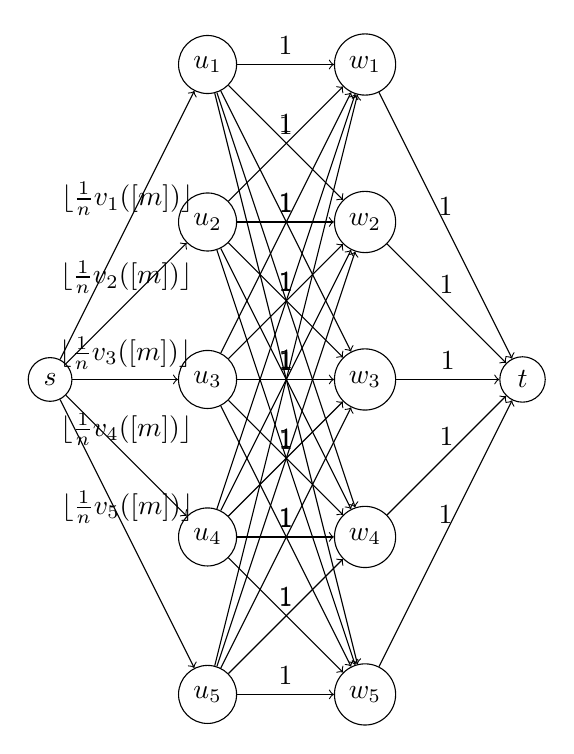
\begin{tikzpicture}
				\node[circle, draw] (s) at (0,0) {$s$};
				\node[circle, draw] (1) at (2,-4) {$u_5$};
				\node[circle, draw] (2) at (2,-2) {$u_4$};
				\node[circle, draw] (3) at (2,0) {$u_3$};
				\node[circle, draw] (4) at (2,2) {$u_2$};
				\node[circle, draw] (5) at (2,4) {$u_1$};
				\node[circle, draw] (w1) at (4,-4) {$w_5$};
				\node[circle, draw] (w2) at (4,-2) {$w_4$};
				\node[circle, draw] (w3) at (4,0) {$w_3$};
				\node[circle, draw] (w4) at (4,2) {$w_2$};
				\node[circle, draw] (w5) at (4,4) {$w_1$};
				\node[circle, draw] (t) at (6,0) {$t$};
				\draw[->] (s) -- (1) node[midway, above] {$\lfloor\frac{1}{n}v_5([m])\rfloor$};\draw[->] (s) -- (2) node[midway, above] {$\lfloor\frac{1}{n}v_4([m])\rfloor$};\draw[->] (s) -- (3) node[midway, above] {$\lfloor\frac{1}{n}v_3([m])\rfloor$};\draw[->] (s) -- (4) node[midway, above] {$\lfloor\frac{1}{n}v_2([m])\rfloor$};\draw[->] (s) -- (5) node[midway, above] {$\lfloor\frac{1}{n}v_1([m])\rfloor$};
				\draw[->] (w1) -- (t) node[midway, above] {$1$};\draw[->] (w2) -- (t)node[midway, above] {$1$};\draw[->] (w3) -- (t)node[midway, above] {$1$};\draw[->] (w4) -- (t)node[midway, above] {$1$};\draw[->] (w5) -- (t)node[midway, above] {$1$};
				\draw[->] (1) -- (w1) node[midway, above] {$1$};\draw[->] (1) -- (w2) node[midway, above] {$1$};\draw[->] (1) -- (w3) node[midway, above] {$1$};\draw[->] (1) -- (w4) node[midway, above] {$1$};\draw[->] (1) -- (w5) node[midway, above] {$1$};
				\draw[->] (2) -- (w1) node[midway, above] {$1$};\draw[->] (2) -- (w2) node[midway, above] {$1$};\draw[->] (2) -- (w3) node[midway, above] {$1$};\draw[->] (2) -- (w4) node[midway, above] {$1$};\draw[->] (2) -- (w5) node[midway, above] {$1$};
				\draw[->] (3) -- (w1) node[midway, above] {$1$};\draw[->] (3) -- (w2) node[midway, above] {$1$};\draw[->] (3) -- (w3) node[midway, above] {$1$};\draw[->] (3) -- (w4) node[midway, above] {$1$};\draw[->] (3) -- (w5) node[midway, above] {$1$};
				\draw[->] (4) -- (w1) node[midway, above] {$1$};\draw[->] (4) -- (w2) node[midway, above] {$1$};\draw[->] (4) -- (w3) node[midway, above] {$1$};\draw[->] (4) -- (w4) node[midway, above] {$1$};\draw[->] (4) -- (w5) node[midway, above] {$1$};
				\draw[->] (5) -- (w1) node[midway, above] {$1$};\draw[->] (5) -- (w2) node[midway, above] {$1$};\draw[->] (5) -- (w3) node[midway, above] {$1$};\draw[->] (5) -- (w4) node[midway, above] {$1$};\draw[->] (5) -- (w5) node[midway, above] {$1$};
			\end{tikzpicture}
			
			Plot 1: solution network
		\end{center}
	
		The time complexity is the one of Edmonds-Karp, and the correctness is proved in the previous parts.
		\end{enumerate}
	\end{ans}
	
	\begin{prob}
		(25 points) [Hall Marriage Theorem] Given a bipartite graph $G=(A, B, E)$ with $|A|=|B|=n$, Hall Marriage Theorem states that $G$ contains a perfect matching (i.e., a matching with size $n$ ) if and only if $|N(S)| \geq|S|$ for any $S \subseteq A$, where $N(S)=\{b \in$ $B \mid \exists a \in S \subseteq A:(a, b) \in E\}$ is the set of all the neighbors of the vertices in $S$. In this question, we are going to prove Hall Marriage Theorem.
		
		\begin{enumerate}[(a)]
			\item (5 points) Prove the necessity part: if $G$ contains a perfect matching, then $|N(S)| \geq$ $|S|$ for any $S \subseteq A$
			\item (10 points) Construct a directed weighted graph with vertex set $V=A \cup B \cup\{s\} \cup$ $\{t\}$. The edge set is defined as follows. For each $a \in A$, construct a directed edge $(s, a)$ with weight 1 ; for each $a \in A$ and $b \in B$, construct a directed edge $(a, b)$ with weight $\infty$ if $(a, b)$ is an edge in the original graph $G$; for each $b \in B$, construct a directed edge $(b, t)$ with weight 1 . Prove that, if $|N(S)| \geq|S|$, the minimum $s$ - $t$ cut has value $n$.
			\item (10 points) Prove the sufficiency part: if $|N(S)| \geq|S|$ holds for all $S \subseteq A$, then $G$ contains a perfect matching.
		\end{enumerate}
	\end{prob}
		
	\begin{ans}
		~
		
		\begin{enumerate}[(a)]
			\item If $G$ contains a perfect match, each vertex in $A$ must attach at least one vertex in $B$. So, for a subset $S$ of $A$, in the perfect match there are $|S|$ vertices in $B$ attached to $S$, which implies $|N(S)| \geq$ $|S|$. Let's prove by contradiction: if $|N(S)| <$ $|S|$, there mustn't be a perfect match.
			\item In this problem, we draw the network like Plot 0 and 1. There are two significant positions: $(a_i, a_{i+1})$, $(b_j, b_{j+1})$ between which the cut line go through. Ignore the cut including only $(s, a_i), (b_j, t) \text{ or }(a_i, b_j)$. These three conditions have flow at least $n$. According to symmetry, we only consider the condition the line start from upper-right. That is: the cut set include $(s, a_1), (s, a_2)\cdots (s, a_i)$, $(b_{j+1}, t), (b_{j+2}, t)\cdots (b_n, t)$ and other edges. When $i\geq j$, the cut of $(s, a_p)$ and $(b_q, t)$ is already larger than n. When $i<j$, the flow include three parts: $(s, a_p)$ with flow i, $(b_q, t)$ with flow $n-j$ and the edges from set $S_A=\{a_{i+1}, a_{i+2}\cdots a_{n}\}\text{ to }S_B=\{b_{1}, b_{2}\cdots b_{j}\}$. Here we have $n-i>n-j$. According to the claim we made in Part (a), $N(S_A)\geq n-i>n-j$, and so there must be at least one edge from $S_A \text{ to } S_B$, causing the cut value to be over $n$. Now we prove the min s-t cut is $n$. 
			\item Like what we've done in Problem 1., we can replace the $\infty$ capacities with $1$, which will not influence the flow. Construct the network like Part (b). Since we know the min cut equals the max flow, we can use Edmonds-Karp to find an integral flow with value $n$. In this flow, each $a_i$ is linked to a unique $b_j$ through an edge with flow 1 on it. This is a required perfect matching.
		\end{enumerate}
	\end{ans}
	
	\begin{prob}
		(25 points) [LP-Duality and Total Unimodularity] In this question, we will prove König-Egerváry Theorem, which states that, in any bipartite graph, the size of the maximum matching equals to the size of the minimum vertex cover. Let $G=(V, E)$ be a bipartite graph.
		
		\begin{enumerate}[(a)]
			\item (4 points) Explain that the following linear program describes the fractional version of the maximum matching problem (i.e., replacing $x_{e} \geq 0$ to $x_{e} \in\{0,1\}$ gives you the exact description of the maximum matching problem).
			$$
			\begin{aligned}
				\text { maximize } & \sum_{e \in E} x_{e} \\
				\text { subject to } & \sum_{e: e=(u, v)} x_{e} \leq 1 & (\forall v \in V) \\
				& x_{e} \geq 0 & (\forall e \in E)
			\end{aligned}
			$$
			\item (4 points) Write down the dual of the above linear program, and justify that the dual program describes the fractional version of the minimum vertex cover problem.
			\item (7 points) Show by induction that the incident matrix of a bipartite graph is totally unimodular. (Given an undirected graph $G=(V, E)$, the incident matrix $A$ is a $|V| \times|E|$ zero-one matrix where $a_{i j}=1$ if and only if the $i$-th vertex and the $j$-th edge are incident.)
			\item (6 points) Use results in (a), (b) and (c) to prove König-Egerváry Theorem.
			\item (4 points) Give a counterexample to show that the claim in König-Egerváry Theorem fails if the graph is not bipartite. 
		\end{enumerate}
	\end{prob}

	\begin{ans}
		~
		
		\begin{enumerate}[(a)]
			\item The description of the problem is ambiguous. I'm not sure what exactly I need to explain. 
			
			If we replace $x_{e} \geq 0$ to $x_{e} \in\{0,1\}$, the new constriction means each edge has only two states: selected or not selected. Each vertex can only be connected to one selected edge. The both ending vertices of a selected edge is a pair, and the result of maximizing the number of selected edges is the max match. 
			
			The fractional version of the problem is: a vertex can be divided into fractional parts and then be matched to different vertices. There restrictions are: the matched part should be in [0,1], represented by the value on an edge $x_e$ and the sum of the part is 1. This liner program describes this problem. 
			
			\item The dual program is 
			
			$$
			\begin{aligned}
				\text { minimize } & \sum_{v \in V} y_{v} \\
				\text { subject to } & \sum_{(v_1,v_2) \in E} y_{v_i} \geq 1 & (\forall e \in E) \\
				& y_{v} \geq 0 & (\forall v \in V)
			\end{aligned}
			$$
			
			We have to explain this is a fractional version of vertex cover. However, I can't see what is a fractional vertex cover. So I guess we have to replace $y_v\geq0 \text{ with } y_v\in\{0,1\}$. Here variable $y_v$ represents whether the vertex is in the vertex cover. $\sum_{(v_1,v_2) \in E} y_{v_i} \geq 1$ means for each edge, at least one end is in the vertex cover. The result of the minimum vertex cover is exactly the minimized $y_v$. 
			
			\item Show by induction:
			
			1. For case $|V|=1$, the incident matrix is obviously totally unimodular. 
			
			2. For other cases, if the incident matrix for bipartite graph with $k-1$ vertices is totally unimodular, discuss the case for $k$.
			
			The $k$ graph $G$ is obtained by adding a $kth$ vertex onto a $k-1$ graph $G'$. According to the induction, the incident matrix $A'$ for $G'$ is unimodular. 
			
			According to the definition of the incident matrix, the incident matrix of $G$ can be written as
			
			$$A = \left(\begin{matrix} A' & E_k \\ \boldsymbol 0 & \boldsymbol 1 \end{matrix}\right)$$
			
			$E_k$ is a matrix representing the additional edges based on $A'$. The square sub-matrices of $A'$ have determinate 0 or $\pm1$. Adding a row with all 0 does not change unimodularity, so the left part of $A$:$\left(\begin{matrix} A'\\ \boldsymbol 0\end{matrix}\right)$ is unimodular. For matrix $\left(\begin{matrix} E_k \\ \boldsymbol 1 \end{matrix}\right)$, the last row is all 1. In $E_k$, there is one and only one 1 in each column. Any sub-matrix of $E_k$ has determinate 0 or $\pm$ 1 because at most one component is non-zero in the determinant calculation formula expanded by column. Since all the element is 0 and $\pm1$, the determinate is 0 or $\pm1$. 
			
			Adding a row with all 1, the right part of $A$ is still unimodular. For sub-matrices across the two part: consider the square matrices with size $|V|$ composed of some columns in $\left(\begin{matrix} A'\\ \boldsymbol 0\end{matrix}\right)$ and some columns in $\left(\begin{matrix} E_k \\ \boldsymbol 1 \end{matrix}\right)$. For sub-matrices in the upper k-1 rows, since $E_k$ has only one 1 in each column and $A'$ is composed of 0 and 1s, the determinate is 0 or $\pm1$. For sub-matrices including the last row, expand the determinate by the last column to get 0 and a determinate of a matrix in the upper k-1 row. Thus A is totally unimodular. 
			
			\item According to the duality of linear programming, the linear program in (a) and (b) share the same solution. The linear program in (a) represent the max matching problem and (b) the min vertex cover problem. Therefore, we have transformed the maximum matching problem into the minimum vertex cover problem, and the minimum vertex cover problem can also be transformed into the maximum matching problem. Thus, we have $|M|=|C|$, which is the König-Egerváry Theorem.
			
			\item Plot 2 shows the example with min vertex cover size 3 but max match 2. 
			\begin{center}
				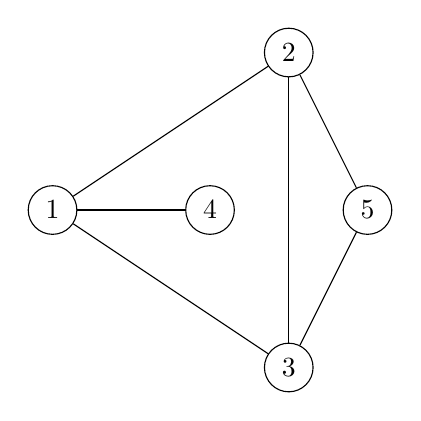
\begin{tikzpicture}
					\node[circle, draw] (1) at (0,0) {$1$};
					\node[circle, draw] (2) at (3,2) {$2$};
					\node[circle, draw] (3) at (3,-2) {$3$};
					\node[circle, draw] (4) at (2,0) {$4$};
					\node[circle, draw] (5) at (4,0) {$5$};
					\draw[-] (1) -- (2);
					\draw[-] (1) -- (3);
					\draw[-] (1) -- (4);
					\draw[-] (3) -- (2);
					\draw[-] (5) -- (2);
					\draw[-] (3) -- (5);
				\end{tikzpicture}
				
				Plot 2: example
			\end{center}
		\end{enumerate}
	\end{ans}

	\begin{prob}
		(25 points) [LP and Vertex Cover] In this question, we are going to design a 2-approximation algorithm for the minimum vertex cover problem that is different from the one learned in the class. Let $G=(V, E)$ be an undirected graph for which we want to find a minimum vertex cover.
		
		\begin{enumerate}[(a)]
			\item (5 points) Explain that the following linear program describes the fractional version of the vertex cover problem (i.e., replacing $x_{u} \geq 0$ to $x_{u} \in\{0,1\}$ gives you the exact description of the minimum vertex cover problem).
			
			$$
			\begin{aligned}
				& \operatorname{minimize} \sum_{u \in V} x_{u} \\
				& \text { subject to } x_{u}+x_{v} \geq 1 \quad(\forall(u, v) \in E) \\
				& x_{u} \geq 0 \quad(\forall u \in V)
			\end{aligned}
			$$
			\item (5 points) Let $\left\{x_{u}^{*}\right\}_{u \in V}$ be an optimal solution to the linear program in Part (a). Prove that $\sum_{u \in V} x_{u}^{*}$ is a lower bound to the size of any vertex cover.
			\item (10 points) Consider the following algorithm.
			
			\begin{itemize}
				\item Solve the linear program in Part (a) and obtain an optimal solution $\left\{x_{u}^{*}\right\}_{u \in V}$;
				
				\item $\operatorname{Return} S=\left\{u \in V \mid x_{u}^{*} \geq 0.5\right\}$.
				
			\end{itemize}
			
			Prove that the algorithm returns a valid vertex cover, and it is a 2-approximation algorithm.
			
			\item (5 points) Show that there exists an integral optimal solution to the linear program in Part (a) if $G$ is a bipartite graph. Notice that an integral optimal solution to this linear program directly gives you a minimum vertex cover. (Hint: This almost straightforwardly follows from one of the previous questions you have solved. Can you see it?)
		\end{enumerate}
	\end{prob}
	
	\begin{ans}
		~
		
		\begin{enumerate}[(a)]
			\item I guess this liner program is the dual program of the last problem, which I explained in (b) in the last problem. 
			
			\item Replace $x_u\geq 0$ with $x_u \in \{0,1\}$. This is a stronger restriction and is included in the original restriction. Suppose the smallest vertex cover has size $s^*$, $\underset{u\in V}{\sum}x_u^{*}$ should be larger than $s^*$ because in the last problem we explained the modified program describes the vertex cover problem and the case $s^*$ is a solution for the modified problem. Since the original program has weaker restriction, the solution should be no larger, and thus is the lower bound. 
			
			\item First prove the solution is valid. Since the program ensures $x_{u}+x_{v} \geq 1$, at least one end will be over 0.5 and selected. This satisfies the definition of vertex cover. Then prove the algorithm is 2-approximate. Suppose the optimal size is $S_{opt}$. $\underset{u \in S}{\sum} x_u^* \geq 0.5 |S|$. Since $\underset{u \in S}{\sum} x_u^*$ is the lower bound of any vertex cover: $\sum_{u \in V} x_u^*\leq |S_{opt}|$. So $|S| \leq 2 \cdot |S_{opt}|$
		\end{enumerate}
	\end{ans}
	
	\begin{prob}
		(Bonus 60 points) [Dinic's Algorithm] In this question, we are going to work out Dinic's algorithm for computing a maximum flow. Similar to Edmonds-Karp algorithm, in each iteration of Dinic's algorithm, we update the flow $f$ by increasing its value and then update the residual network $G^{f}$. However, in Dinic's algorithm, we push flow along multiple $s$ - $t$ paths in the residual network instead of a single $s$ - $t$ path as it is in Edmonds-Karp algorithm.
		
		In each iteration of the algorithm, we find the level graph of the residual network $G^{f}$. Given a graph $G$ with a source vertex $s$, its level graph $\bar{G}$ is defined by removing edges from $G$ such that only edges pointing from level $i$ to level $i+1$ are kept, where vertices at level $i$ are those vertices at distance $i$ from the source $s$. An example of level graph is shown in Fig. 1.
		
		Next, the algorithm finds a blocking flow on the level graph $\bar{G}^{f}$ of the residual network $G^{f}$. A blocking flow $f$ in $G$ is a flow such that each $s$ - $t$ path contains at least one critical edge. Recall that an edge $e$ is critical if the amount of flow on it reaches its capacity: $f(e)=c(e)$. Fig. 2 gives examples for blocking flow.
		
		Dinic's algorithm is then described as follows.
		
		\begin{enumerate}
			\item Initialize $f$ to be the empty flow, and $G^{f}=G$.
			
			\item Do the following until there is no $s-t$ path in $G^{f}$ :
		
			\begin{itemize}
				\item construct the level graph $\bar{G}^{f}$ of $G^{f}$.
				
				\item find a blocking flow on $\bar{G}^{f}$.
				
				\item Update $f$ by adding the blocking flow to it, and update $G^{f}$.
				
			\end{itemize}
		\end{enumerate}
	
		Complete the analysis of Dinic's algorithm by solving the following questions.
		
		\begin{enumerate}[(a)]
			\item (15 points) Prove that, after each iteration of Dinic's algorithm, the distance from $s$ to $t$ in $G^{f}$ is increased by at least 1 .
			\item (15 points) Design an $O(|V| \cdot|E|)$ time algorithm to compute a blocking flow on a level graph.
			\item (10 points) Show that the overall time complexity for Dinic's algorithm is $O(|V|^{2}\cdot|E|)$
			\item (20 points) (challenging) We have seen in the class that the problem of finding a maximum matching on a bipartite graph can be converted to the maximum flow problem. Show that Dinic's algorithm applied to finding a maximum matching on a bipartite graph only requires time complexity $O(|E| \cdot \sqrt{|V|})$.
		\end{enumerate}

		\begin{center}
			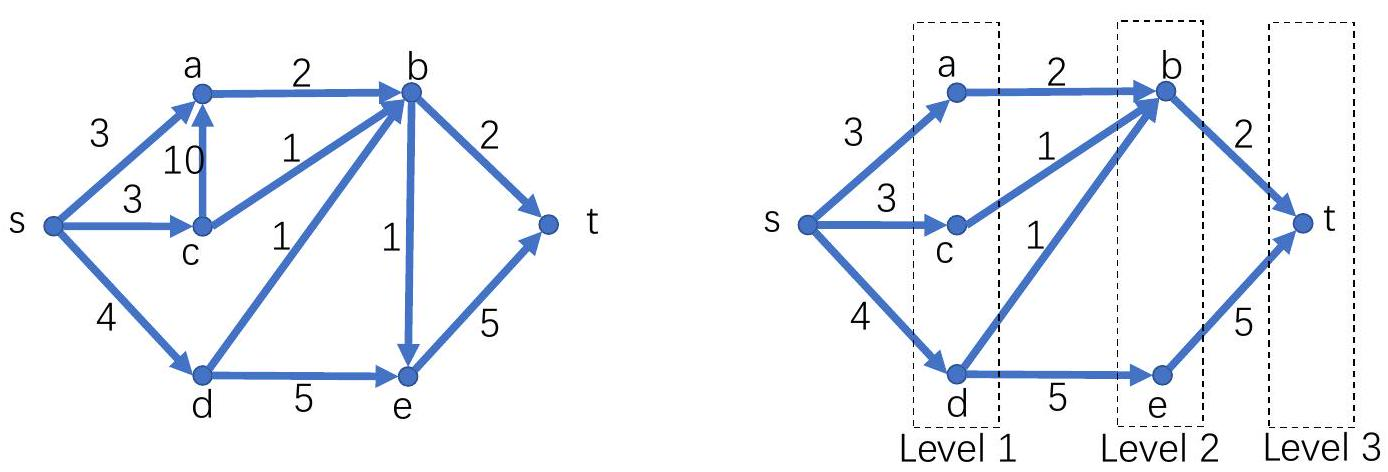
\includegraphics[width=\textwidth,]{images/2022_12_05_f18b1b761080a7308df7g-6}
		\end{center}
	
		Figure 1: The graph shown on the right-hand side is the level graph of the graph on the left-hand side. Only edges pointing to the next levels are kept. For example, the edges $(c, a)$ and $(b, e)$ are removed, as they point at vertices at the same level. If there were edges pointing at previous levels, they should also be removed.

		\begin{center}
			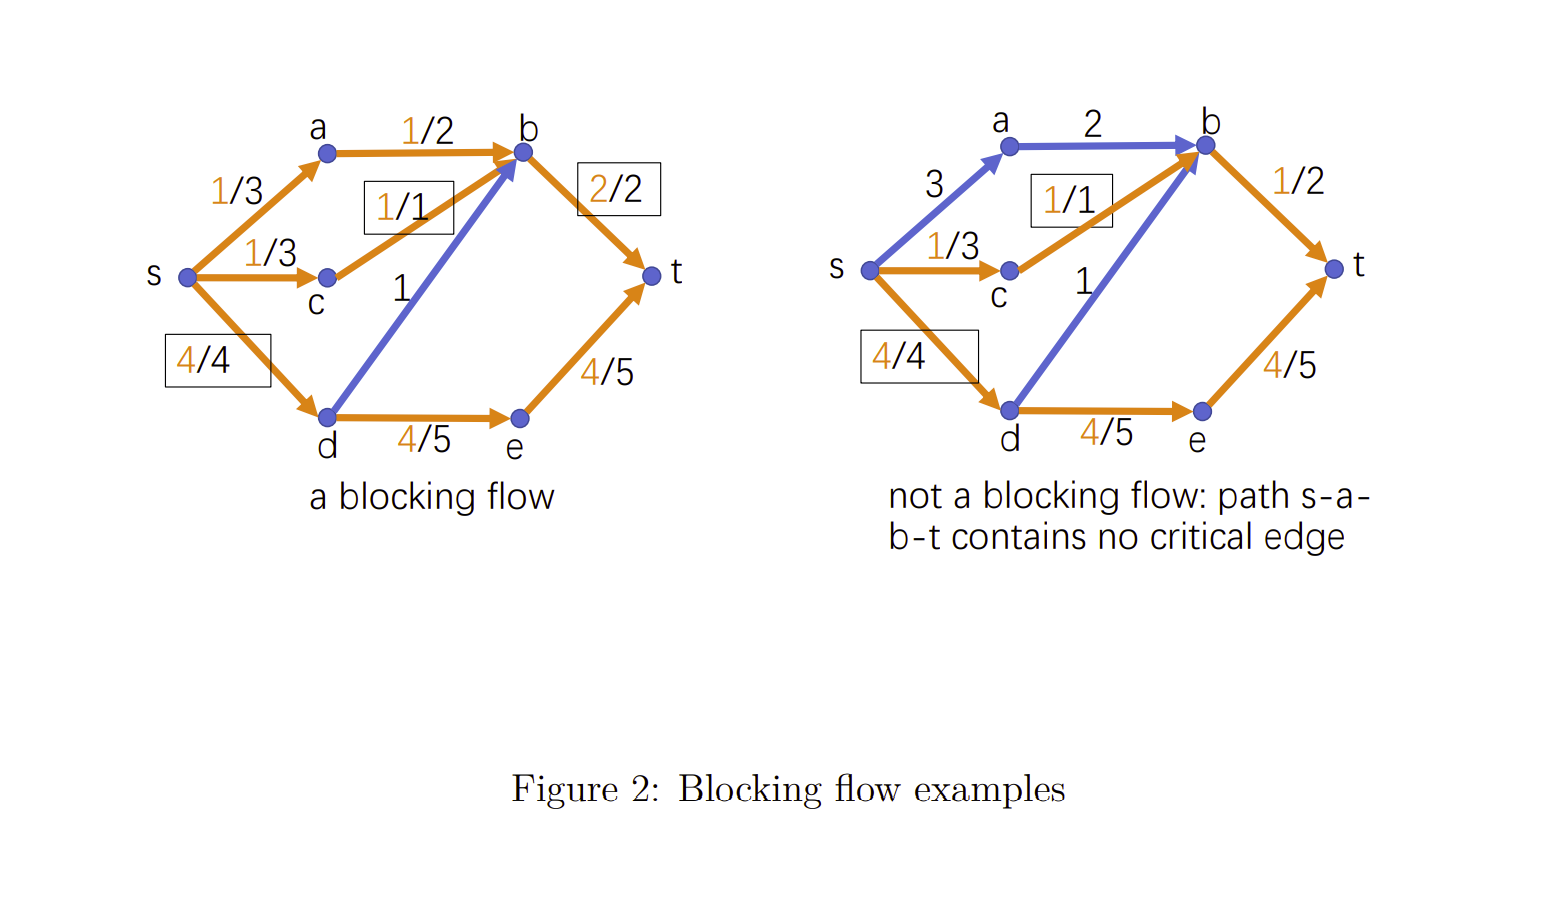
\includegraphics[width=\textwidth]{images/6}
		\end{center}		

	
	\end{prob}	
	~
	
	It's a pity that we vegetables are too busy by the end of the term. I will finish it as short.	
	\begin{enumerate}[(a)]
		\item The level is defined by the distance from s to a vertex i. If the s-t distance k does not increase after an iteration, it means there is still a s-t path with k. Since before the update the vertex t is k-level, this s-t path is also in $\bar{G^f}$: each vertex on the path is different level. However, during the iteration, the update rule requires us to find the critical path on this s-t path, which means after the update, this s-t path shouldn't exist. 
		
		\item We can use DFS to find all the route and record the min capacity. The min capacity is updated both when going to successors and returning to predecessors. When DFS, you can only go to and return back from each vertex once, and so there are at most $O(n)$ moves forward and backward. Each DFS will cause at least one pair of vertices to disconnect, and there are $O(|E|)$ DFSs. The time complexity is $O(|V|\cdot |E|)$ and it ensures in the $\bar{G^F}$ there are no more s-t path. 
		
		\item There are $|V|$ vertices so there are initially at most $|V|$ levels. Each update is $O(|V|\cdot |E|)$ and the level will reduce by 1. The total complexity is $O(|V|^{2}\cdot|E|)$
		
		\item I will skip it for now. If I have time in the future.
		
	\end{enumerate}
	
	\begin{prob}
		How long does it take you to finish the assignment (including thinking and discussing)? Give a score $(1,2,3,4,5)$ to the difficulty. Do you have any collaborators? Write down their names here.
	\end{prob}

	\begin{ans}
		~
		
		Difficult score 3. My collaborator is chatGPT. However, I only use it to confirm my thoughts.
	\end{ans}
\end{document}
